\begin{figure}[ht]
    \centering

    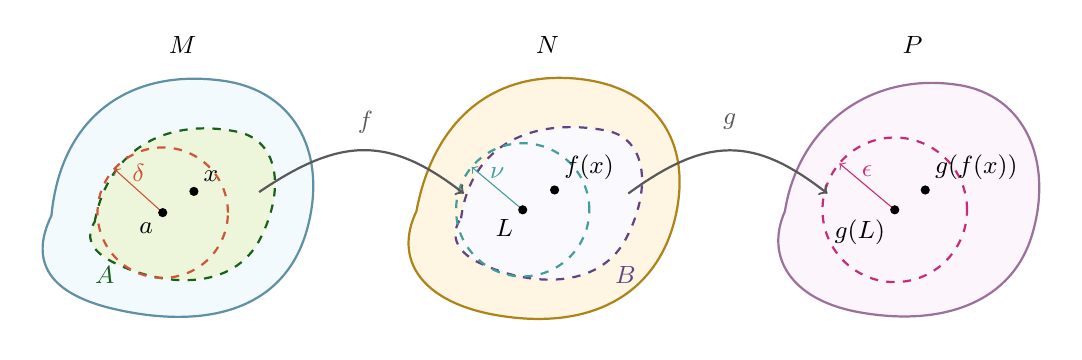
\begin{tikzpicture}[
        scale=0.9,
        every node/.style={font=\small},
        mspace/.style={fill=SkyBlue!10, draw=SkyBlue!70!black, thick},
        nspace/.style={fill=Dandelion!12, draw=Goldenrod!80!black, thick},
        pspace/.style={fill=Plum!10, draw=Plum!70!black, thick},
        asubspace/.style={fill=YellowGreen!18, draw=ForestGreen!70!black, thick, dashed},
        bsubspace/.style={fill=Lavender!20, draw=RoyalPurple!72!black, thick, dashed},
        map/.style={->, thick, black!65},
        margin/.style={thick, dashed}
    ]
        \begin{scope}
            \path[mspace]
                (-1.85,-0.16)
                .. controls (-1.72,1.22) and (-0.76,1.93) .. (0.58,1.74)
                .. controls (1.63,1.59) and (2.05,0.66) .. (1.75,-0.38)
                .. controls (1.42,-1.52) and (0.30,-1.76) .. (-0.92,-1.49)
                .. controls (-1.88,-1.28) and (-2.17,-0.82) .. (-1.85,-0.16)
                -- cycle;
            \node at (0,2.24) {$M$};

            \path[asubspace]
                (-1.24,-0.25)
                .. controls (-1.04,0.82) and (-0.18,1.22) .. (0.78,1.02)
                .. controls (1.37,0.89) and (1.44,0.19) .. (1.10,-0.48)
                .. controls (0.72,-1.23) and (-0.26,-1.18) .. (-0.98,-0.82)
                .. controls (-1.31,-0.65) and (-1.37,-0.46) .. (-1.24,-0.25)
                -- cycle;
            \node[ForestGreen!70!black] at (-1.10,-1.00) {$A$};

            \coordinate (a) at (-0.28,-0.12);
            \coordinate (x) at (0.16,0.18);
            \coordinate (Aedge) at (1.08,0.17);

            \draw[margin, RedOrange!82!black] (a) circle (0.92);
            \draw[RedOrange!82!black, ->] (a) -- ++(138:0.92)
                node[midway, above] {$\delta$};
            \filldraw[black] (a) circle (1.6pt) node[below left] {$a$};
            \filldraw[black] (x) circle (1.6pt) node[above right] {$x$};
        \end{scope}

        \begin{scope}[xshift=5.15cm]
            \path[nspace]
                (-1.85,-0.10)
                .. controls (-1.62,1.13) and (-0.82,1.89) .. (0.42,1.77)
                .. controls (1.63,1.65) and (2.05,0.77) .. (1.79,-0.24)
                .. controls (1.52,-1.27) and (0.62,-1.79) .. (-0.70,-1.57)
                .. controls (-1.77,-1.39) and (-2.18,-0.79) .. (-1.85,-0.10)
                -- cycle;
            \node at (0,2.24) {$N$};

            \path[bsubspace]
                (-1.22,-0.20)
                .. controls (-1.08,0.85) and (-0.20,1.23) .. (0.82,1.04)
                .. controls (1.42,0.93) and (1.47,0.19) .. (1.10,-0.50)
                .. controls (0.72,-1.20) and (-0.24,-1.18) .. (-0.98,-0.82)
                .. controls (-1.30,-0.66) and (-1.38,-0.42) .. (-1.22,-0.20)
                -- cycle;
            \node[RoyalPurple!72!black] at (1.10,-1.00) {$B$};

            \coordinate (L) at (-0.35,-0.08);
            \coordinate (fx) at (0.10,0.20);
            \coordinate (Bin) at (-1.18,0.15);
            \coordinate (Bout) at (1.14,0.15);

            \draw[margin, TealBlue!80!black] (L) circle (0.94);
            \draw[TealBlue!80!black, ->] (L) -- ++(140:0.94)
                node[midway, above] {$\nu$};
            \filldraw[black] (L) circle (1.6pt) node[below left] {$L$};
            \filldraw[black] (fx) circle (1.6pt) node[above right] {$f(x)$};
        \end{scope}

        \begin{scope}[xshift=10.30cm]
            \path[pspace]
                (-1.80,-0.10)
                .. controls (-1.61,1.10) and (-0.60,1.88) .. (0.66,1.68)
                .. controls (1.59,1.53) and (1.98,0.61) .. (1.70,-0.39)
                .. controls (1.42,-1.41) and (0.39,-1.74) .. (-0.78,-1.52)
                .. controls (-1.73,-1.34) and (-2.08,-0.73) .. (-1.80,-0.10)
                -- cycle;
            \node at (0,2.24) {$P$};

            \coordinate (gL) at (-0.25,-0.08);
            \coordinate (gfx) at (0.18,0.20);
            \coordinate (Pedge) at (-1.20,0.15);

            \draw[margin, RubineRed!80!black] (gL) circle (1.02);
            \draw[RubineRed!80!black, ->] (gL) -- ++(140:1.02)
                node[midway, above] {$\epsilon$};
            \filldraw[black] (gL) circle (1.6pt) node[below left] {$g(L)$};
            \filldraw[black] (gfx) circle (1.6pt) node[above right] {$g(f(x))$};
        \end{scope}

        \draw[map] (Aedge) .. controls (2.24,0.96) and (2.92,0.96) .. (Bin);
        \node[black!65] at (2.58,1.16) {$f$};

        \draw[map] (Bout) .. controls (7.40,0.96) and (8.06,0.96) .. (Pedge);
        \node[black!65] at (7.72,1.16) {$g$};
    \end{tikzpicture}

    \caption{Ilustração da demonstração da Proposição~\ref{prop:composicaoLimites}.}
    \label{fig:composicao}
\end{figure}